\documentclass{ctexart}
\usepackage{upgreek}
\usepackage[a4paper,margin=2.5cm]{geometry}
\usepackage{theorem}
{
	\theoremstyle{change}
	\theoremheaderfont{\bfseries}
	\theorembodyfont{\normalfont}
	\newtheorem{ti}{}[section]
}
\renewcommand{\theti}{\arabic{ti}.}
\usepackage{siunitx}
\usepackage{hyperref}
\setlength{\headheight}{13pt}
\usepackage{fancyhdr}
\pagestyle{fancy}
\fancyhf{}
\fancyhead[C]{江理学习资料库:\mbox{\url{https://github.com/sikouhjw/jxust-Learning-database}}}
\fancyfoot[C]{\thepage}
\usepackage[siunitx,RPvoltages]{circuitikz}
\usepackage{tikz}
\usetikzlibrary{positioning}
% \usetikzlibrary{positioning,shapes.geometric,calc}
% \newcommand*{\circled}[1]{\lower.7ex\hbox{\tikz\draw (0pt, 0pt)%
% 	circle (.5em) node {\makebox[1em][c]{\small #1}};}}
\ctexset{
	section={
		name={,、},
		number=\chinese{section},
		aftername={\hspace{0pt}},
	}
}
\setCJKmainfont[Mapping = fullwidth-stop]{SourceHanSerifCN-Regular}
\def\theenumi{\arabic{enumi}}
\def\labelenumi{(\theenumi)}
% \def\labelenumi{\circled{\theenumi}}
\newcommand{\kuo}{\mbox{(\hspace{1pc})}}
\newcommand{\fourch}[4]{\\\begin{tabular}{*{4}{@{}p{3.945cm}}}\texttt{A}.~#1 & \texttt{B}.~#2 & \texttt{C}.~#3 & \texttt{D}.~#4\end{tabular}} % 一行
\newcommand{\twoch}[4]{\\\begin{tabular}{*{2}{@{}p{7.89cm}}}\texttt{A}.~#1 & \texttt{B}.~#2\end{tabular}\\\begin{tabular}{*{2}{@{}p{7.89cm}}}\texttt{C}.~#3 & \texttt{D}.~#4\end{tabular}}  %两行
\newcommand{\onech}[4]{\\\texttt{A}.~#1 \\ \texttt{B}.~#2 \\ \texttt{C}.~#3 \\ \texttt{D}.~#4}  % 四行
\newcommand{\threech}[3]{\\\begin{tabular}{*{3}{@{}p{5.26cm}}}\texttt{A}.~#1 & \texttt{B}.~#2 & \texttt{C}.~#3 \end{tabular}}  % 四行
\newcommand{\hua}[1]{\CJKunderline{\hspace{0.25pc}\phantom{#1}\hspace{0.25pc}}}

\title{《高频电子线路》样卷}
\author{秦舒雅}
\begin{document}
\maketitle
\section{选择题}
\begin{ti}
	功率放大电路与电压放大电路的区别是\kuo
	\twoch{前者比后者电源电压高}{前者比后者电压放大倍数大}{前者比后者效率高}{前者比后者失真小}
\end{ti}

\begin{ti}
	以下哪种信号携带有调制信号的信息\kuo
	\threech{载波信号}{本振信号}{已调波信号}
\end{ti}

\begin{ti}
	小信号谐振放大器的主要技术指标不包括\kuo
	\fourch{电压增益}{失真系数}{通频带}{选择性}
\end{ti}

\begin{ti}
	丙类谐波功率放大器的谐振回路调谐于哪个分量?\kuo
	\fourch{基波}{二次谐波}{其它高次谐波}{直流分量}
\end{ti}

\begin{ti}
	功率放大电路根据以下哪种说法可分为甲类、甲乙类、乙类、丙类等\kuo
	\twoch{电路特点}{功率放大倍数}{电流大小}{功放管静态工作点选择情况}
\end{ti}

\begin{ti}
	在调谐放大器的 LC 回路两端并上一个电阻 $R$,可以\kuo
	\fourch{提高回路的 $Q$ 值}{提高谐振频率}{加宽通频带}{减小通频带}
\end{ti}

\begin{ti}
	高频小信号调谐放大器主要工作在\kuo
	\fourch{甲类}{乙类}{甲乙类}{丙类}
\end{ti}

\begin{ti}
	调幅波的信息包含在它的\kuo
	\threech{频率变化之中}{幅度变化之中}{相位变化之中}{}
\end{ti}

\begin{ti}
	并联谐振回路外加信号频率等于回路谐振频率时,回路呈\kuo
	\fourch{感性}{容性}{阻性}{容性或感性}
\end{ti}

\begin{ti}
	丙类高频功率放大器的通角\kuo
	\fourch{$\theta = 180^\circ$}{$90^\circ < \theta < 180^\circ$}{$\theta = 90^\circ$}{$\theta < 90^\circ$}
\end{ti}

\section{填空题}
\begin{ti}
	无论是调频信号还是调相信号,它们的 $\omega(t)$ 和 $\phi(t)$ 都同时受到调变,其区别仅在于按调制信号规律线性变化的物理量不同,这个物理量在调相信号中是 \hua{相角},在调频信号中是 \hua{频率}。
\end{ti}

\begin{ti}
	小信号谐振放大器的主要特点是以 \hua{谐振回路} 作为放大器的交流负载,具有 \hua{放大} 和 \hua{选频} 功能。
\end{ti}

\begin{ti}
	单调谐放大器经过级联后电压增益 \hua{增大}、通频带 \hua{变窄}。(在空格中填写变化趋势)
\end{ti}

\begin{ti}
	通常将携带有信息的电信号称为 \hua{基带信号},未调制的高频振荡信号称为 \hua{载波},通过调制后的高频振荡信号称为 \hua{调制信号}。
\end{ti}

\begin{ti}
	小信号谐振放大器的主要特点是以 \hua{调谐回路} 作为放大器的交流负载,具有 \hua{放大} 和 \hua{选频} 功能。
\end{ti}

\begin{ti}
	为实现电信号的有效传输,无线电通信通常要进行调制。常用的模拟调制方式可以分为 \hua{调幅}、\hua{调频} 和 \hua{调相} 三种。
\end{ti}

\begin{ti}
	丙类谐振功率放大器根据集电极电流波形的不同,可分为三种工作状态,分别为 \hua{欠压} 状态、\hua{临界} 状态、\hua{过压} 状态;欲使功率放大器高效率输出最大功率,应使放大器工作在 \hua{临界} 状态。
\end{ti}

\begin{ti}
	调谐放大器工作不稳定的主要因素是 \hua{反向传输导纳}。提高调谐放大器稳定性的措施通常采用 \hua{中和法} 和 \hua{失配法}。
\end{ti}

\begin{ti}
	高频谐振功率放大器的工作原理是:当输入信号为余弦波时,其集电极电流是 \hua{周期性余弦} 波,根据集电极电流波形的不同,可分为三种工作状态,分别为 \hua{欠压} 状态、\hua{过压} 状态、\hua{临界} 状态。
\end{ti}


\section{大题}
\begin{ti}
	以下是调幅发射机的原理框图,根据其工作原理分别填写整机框图中的各单元名称。
	\begin{center}
		\begin{tikzpicture}
			\node[fill=white,draw=black] (a) at (0,0) {\phantom{\large 主振}};
			\node[fill=white,draw=black,right=1 of a] (b) {\phantom{\large 倍频器}};
			\node[fill=white,draw=black,right=1 of b] (c) {\phantom{\large 放大器}};
			\node[fill=white,draw=black,right=1 of c] (d) {\phantom{\large 调制}};
			\draw (b) ++ (0,-2) node (e) {} circle (0.2);
			\draw (e) ++ (0.2,0) ++ (0,-0.2) -- ++ (0,0.4);
			\node[above=5pt] at (e) {话筒};
			\node[fill=white,draw=black,right=1.85 of e] (f) {\phantom{\large 放大}};
			\draw[-latex] (a) -- node[below] {a} (b);
			\draw[-latex] (b) -- node[below] {b} (c);
			\draw[-latex] (c) -- node[below] {c} (d);
			\draw[-latex] (e) ++ (0.2,0) -- (f);
			\draw[-latex] (f) -| node[right] {e} (d);
			\draw[-latex] (d) -- node[below] {d} ++ (1.5,0);
			\draw (d) ++ (1.5,0) -- ++ (0,0.8) ++ (0,-0.3) -- ++ (60:0.3) ++ (-120:0.3) -- ++ (120:0.3);
		\end{tikzpicture}
	\end{center}
\end{ti}

\begin{ti}
	在谐振功率放大电路中,若 $V_{\mathrm{bm}}$、$V_{\mathrm{cm}}$ 及 $V_{\mathrm{cc}}$ 不变,而当 $V_{\mathrm{BB}}$ 改变时,$I_{\mathrm{c}1}$ 有明显的变化,问放大器此时工作在何种状态?为什么?
\end{ti}

\begin{ti}
	\begin{enumerate}
		\item 试画出石英谐振器的电路符号、等效电路;
		\item 石英晶片之所以能做成谐振器是因为它具有什么特性?
	\end{enumerate}
\end{ti}

\begin{ti}
	某谐振功率放大器的转移特性如图所示。已知该放大器采用晶体管的参数为:管子的 $V_{\mathrm{BZ}} = \SI{0.6}{V}$,放大器的负偏置 $|V_{\mathrm{BB}}| = \SI{1.4}{V}$,$\theta_{\mathrm{c}} = 70^\circ$,$\cos 70^\circ = 0.342$,$\alpha_{1}(70^\circ) = 0.436$,$\alpha_{0}(70^\circ) = 0.253$,$V_{\mathrm{CC}} = \SI{24}{V}$,$\xi = 0.9$,试计算输出功率、集电极效率。
	\begin{center}
		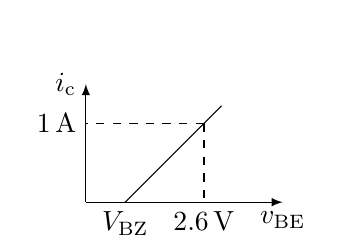
\begin{tikzpicture}
			\draw[-latex] (0,0) -- (2.5,0) node[below] {$v_{\mathrm{BE}}$};
			\draw[-latex] (0,0) -- (0,1.5) node[left] {$i_{\mathrm{c}}$};
			\draw (0.5,0) node[below] {$V_{\mathrm{BZ}}$} -- ++ (45:{sqrt(3)});
			\draw[dashed] (1.5,1) -- (1.5,0) node[below] {\SI{2.6}{V}};
			\draw[dashed] (1.5,1) -- (0,1) node[left] {\SI{1}{A}};
		\end{tikzpicture}
	\end{center}
\end{ti}

\begin{ti}
	设一放大器以简单并联振荡回路为负载,信号中心频率 $f_{s} = \SI{10}{MHz}$,回路电容 $C = \SI{50}{\pF}$,试求:
	\begin{enumerate}
		\item 计算所需的线圈电感值;
		\item 若品质因数为 $Q = 100$,计算回路谐振电阻及回路带宽;
		\item 若放大器所需的带宽 $B = \SI{0.5}{MHz}$,则应在回路上并联多大电阻才能满足放大器所需带宽要求?
	\end{enumerate}
\end{ti}

\begin{ti}
	小信号谐振放大器与谐振功率放大器的主要区别是什么?
\end{ti}

\begin{ti}
	已知某一并联谐振回路的谐振频率 $f_{0} = \SI{1}{MHz}$,要求对 \SI{990}{kHz} 的干扰信号有足够的衰减,试求该并联电路的 $Q$ 值应满足什么条件?
\end{ti}

\begin{ti}
	如下图所示。已知 $L = \SI{0.8}{\upmu H}$,$Q_{0} = 100$,$C_{1} = C_{2} = \SI{20}{\pF}$,$C_{i} = \SI{5}{\pF}$,$R_{i} = \SI{10}{\kilo\ohm}$,$C_{0} = \SI{20}{\pF}$,$R_{0} = \SI{5}{\kilo\ohm}$。试计算回路谐振频率,谐振阻抗(不计 $R_{0}$ 和 $R_{i}$ 时)、有载 $Q_{\mathrm{L}}$ 值和通频带。
	\begin{center}
		\begin{circuitikz}[european]
			\ctikzset{inductor=american}
			\draw (0,0) to[C,C=$C_{i}$] (0,4) -- (2,4) to[R,R=$R_{i}$,*-*] (2,0) -- (0,0);
			\draw (2,4) -- (4,4) to[L,L=$L$,*-*] (4,0) -- (2,0);
			\draw (4,4) -- ++ (2,0) to[C,C=$C_{1}$,-*] ++ (0,-2) to[C,C=$C_{2}$,-*] ++ (0,-2) -- ++ (-2,0);
			\draw (6,2) -- ++ (2,0) to[R,R=$R_{0}$,*-*] ++ (0,-2) -- ++ (-2,0);
			\draw (8,2) -- ++ (2,0) to[C,C=$C_{0}$] ++ (0,-2) -- ++ (-2,0);
		\end{circuitikz}
	\end{center}
\end{ti}

\begin{ti}
	某非线性器件的伏安特性为 $i = a_{1} u + a_{3} u^{3}$,试问该器件能否实现相乘作用?为什么?
\end{ti}

\begin{ti}
	小信号谐振放大器与谐振功率放大器的主要区别是什么?
\end{ti}

\begin{ti}
	一个 \SI{5}{\upmu H} 的线圈与一个可变电容相串联,外加电压值与频率是固定的。当 $C = \SI{126.6}{\pF}$ 时,电路电流达到最大值 \SI{1}{A}。当 $C = \SI{100}{\pF}$ 时,电流减为 \SI{0.5}{A}。
	\begin{enumerate}
		\item 电源频率;
		\item 电路的 $Q$ 值;
		\item 外加电压数值。
	\end{enumerate}
\end{ti}

\begin{ti}
	某一晶体管谐振功率放大器,设已知 $V_{\mathrm{CC}} = \SI{22}{V}$,$I_{\mathrm{C}0} = \SI{200}{mA}$,$P_{0} = \SI{4}{W}$,电压利用系数 $\xi = 1$。求:$P_{=}$、$\eta_{\mathrm{C}}$、$R_{\mathrm{P}}$、$I_{\mathrm{cm}1}$。
\end{ti}
\end{document}